\section{Elaboration of the example}
\label{sec:elaboration}

An example graph query is shown in \figref{patterndef} %(the query is intentionally domain-independent to emphasize the generalizability of the approach), 
as a graph pattern definition in \eiq{} syntax~\cite{models10} on the left and graphically on the right. This query represents a typical pattern that is used in MDE applications (such as well-formedness validation or complex model transformations), whereby a subgraph of 4 connected vertices ($V1, V2, V3, V4$) is sought after with a \emph{negative application condition} prescribing that a typed edge (between vertices $V4$ and $V1$) must not exist.
The Rete network constructed for matching this graph pattern is depicted in \figref{retelayout}. In \iqd{}, type-instance indexers for edge types enumerate all source and target vertices, thus the intermediate join nodes perform join operations on vertex pairs that are connected by typed edges as prescribed by the definition in \figref{patterndef}. The join nodes all store the intermediate query results (e.g.\ connected $V1-V2$ and $V2-V3$ tuples in the case of the leftmost join node), and keep these caches up-to-date as change tokens arrive from the middleware (whenever model changes are performed).

\emph{Information representation and distributed operation.} The Rete layer of \iqd{} is \emph{domain and storage agnostic} as it stores only tuples constructed from model element identifiers and literals, thus it can be used independently of the model representation format (metamodeling language) of the model repository.
As illustrated in \figref{architecture}, the Rete nodes can be allocated to different hosts in a cloud computing infrastructure (as the communication protocol supports remoting). As change propagation is asynchronous, \iqd{} implements a \emph{termination protocol} to ensure that the query results can be retrieved consistently with the model state after a given transaction (i.e.\ by signaling when the update propagation has been terminated).

% \begin{figure}[!tb]
% \begin{center}
% 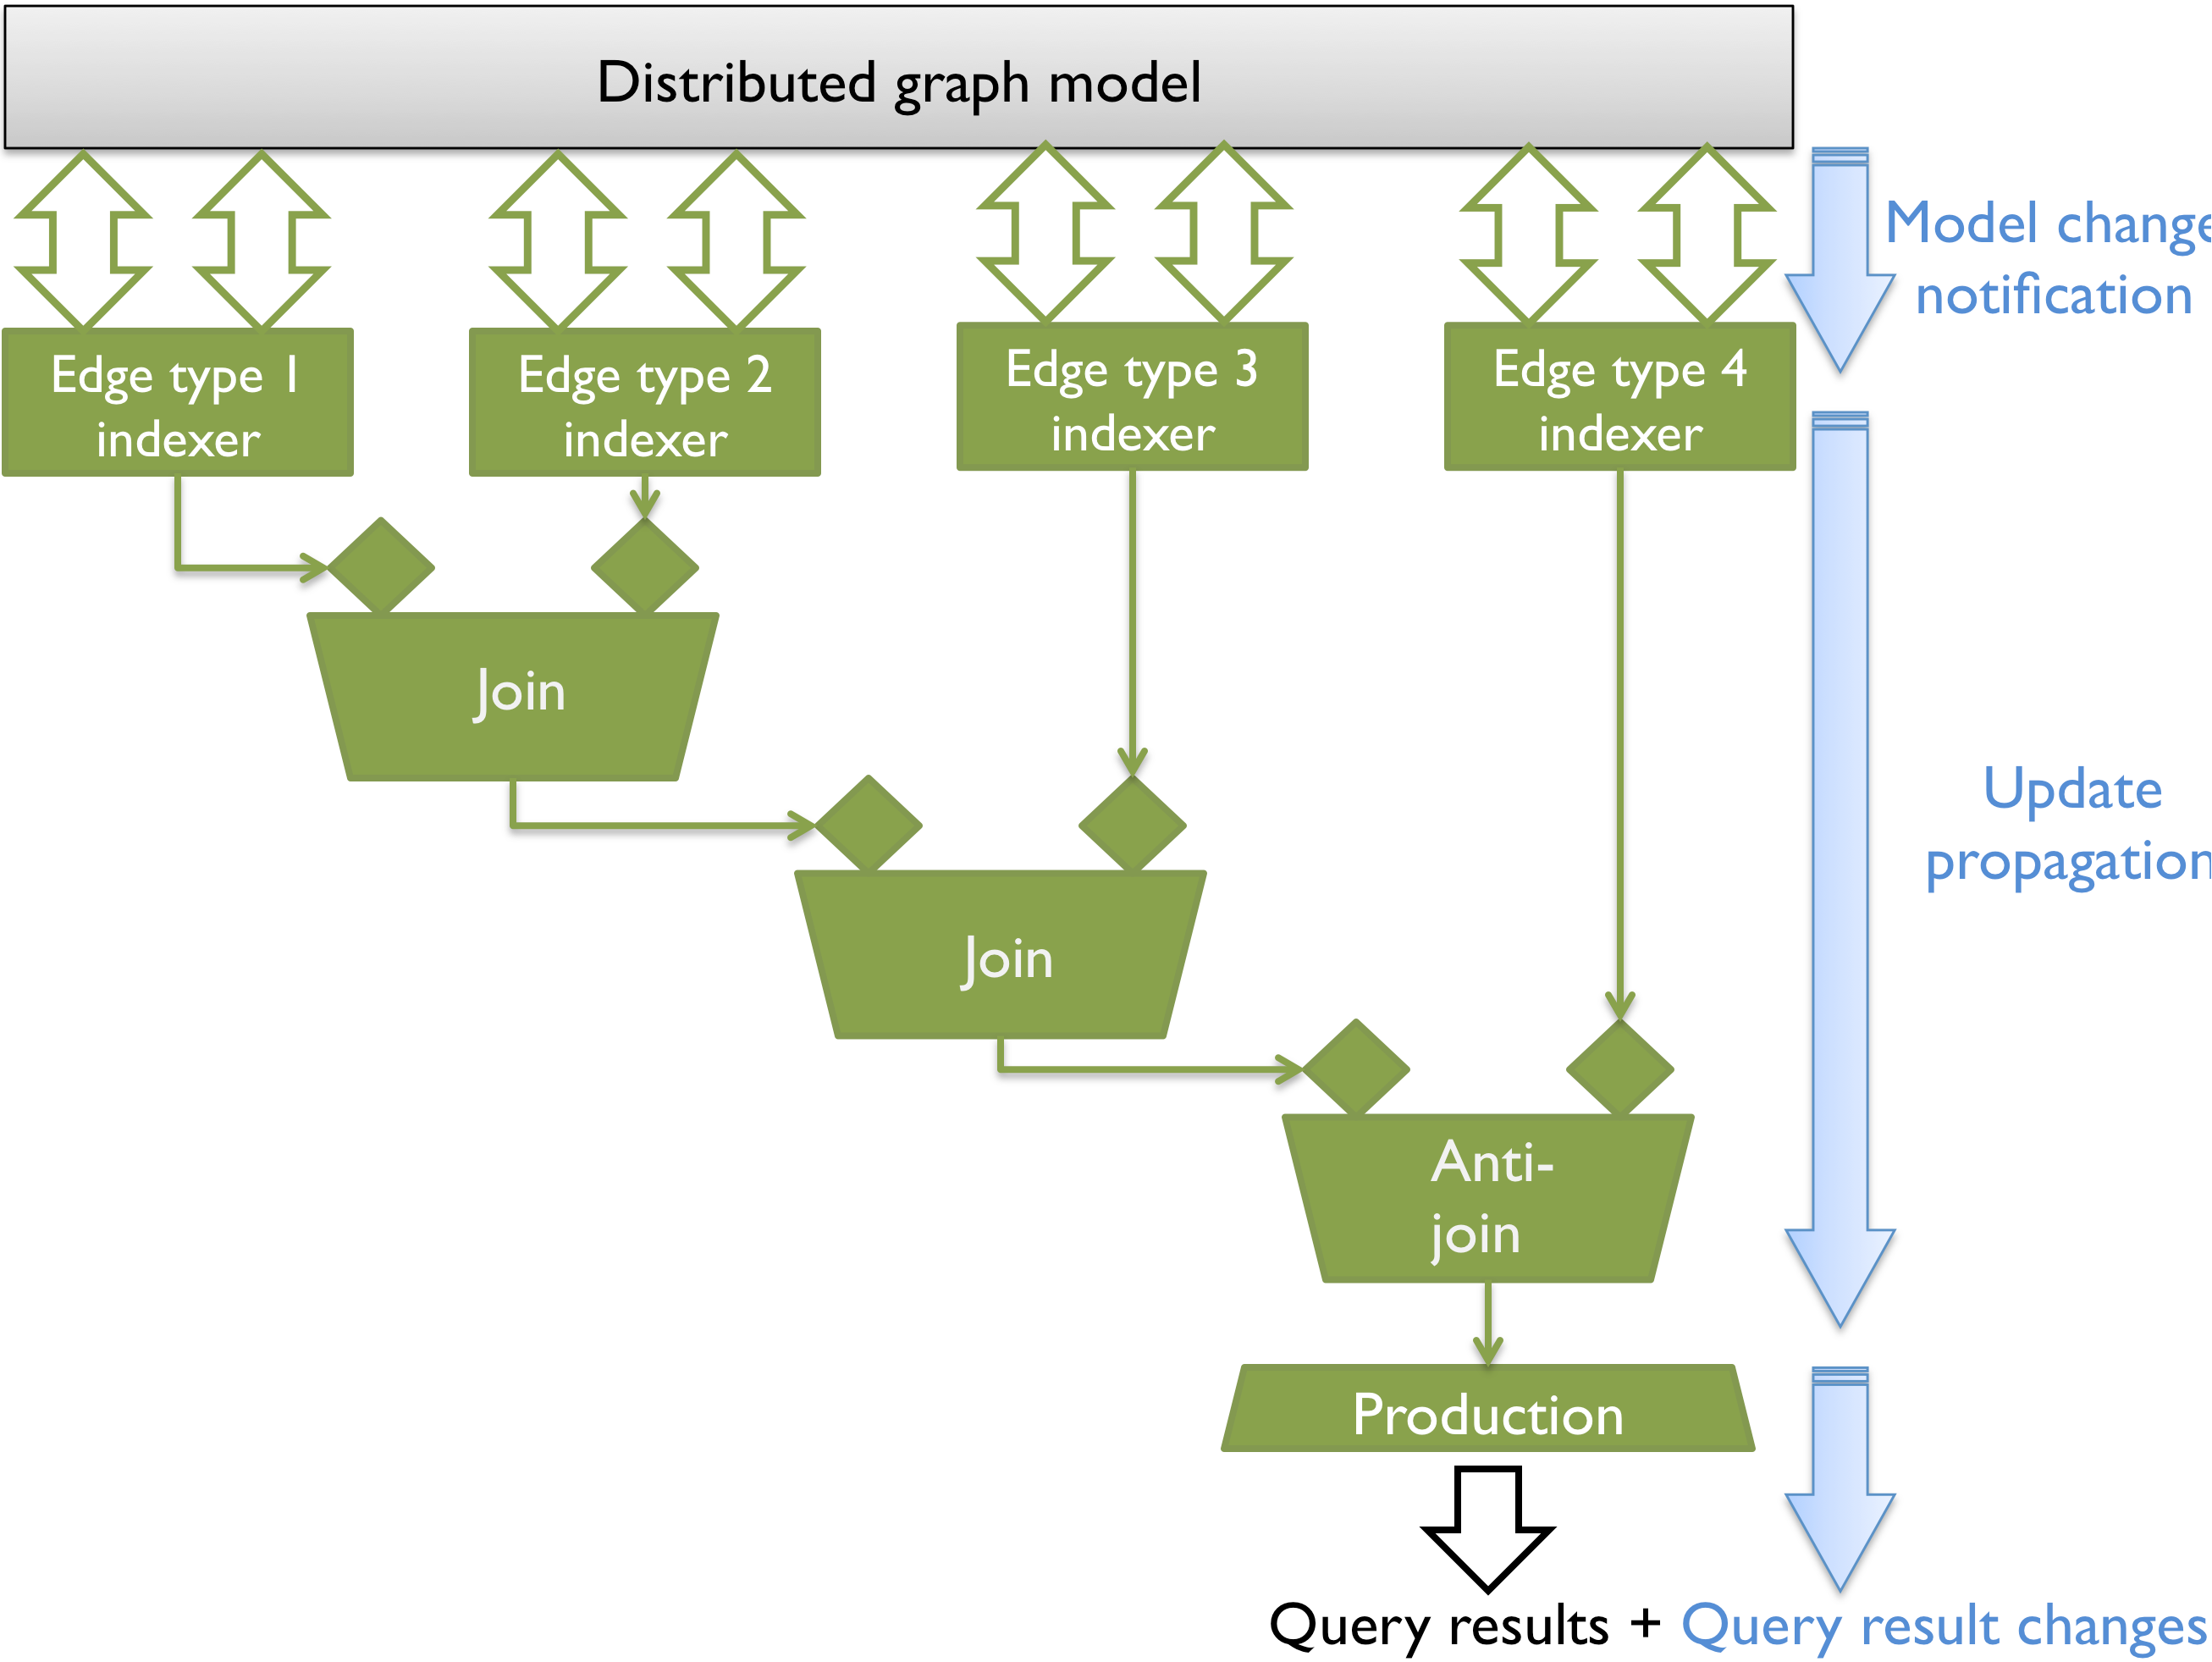
\includegraphics[width=.8\columnwidth]{figures/reteinternals}
% \caption{Rete layout}
% \label{fig:retelayout}
% \end{center}
% \end{figure}
